\documentclass[12pt]{report}
\setcounter{secnumdepth}{5}
\usepackage[utf8]{inputenc}
\usepackage{amsmath,amsfonts,amssymb}
\usepackage{mathtools}
\DeclarePairedDelimiter{\ceil}{\lceil}{\rceil}
\usepackage{graphicx}
\usepackage{float}
\usepackage{listings}
\usepackage{bbm}
\usepackage{indentfirst}
\usepackage{blindtext}
\usepackage{titlesec}
\usepackage[utf8]{inputenc}
\usepackage{listings}
\usepackage{braket}
\usepackage{tikz}
\usetikzlibrary{quantikz}
\usepackage{algorithm}
\usepackage{algorithmic}
\usepackage[english]{babel}
\usepackage{xcolor}
\usepackage{MnSymbol,wasysym}
\usepackage{hyperref}
\usepackage{graphicx}
\usepackage{amsmath}
\usepackage{braket}
\graphicspath{ {images/}}
\usepackage[style=numeric]{biblatex}
\addbibresource{thesis.bib}




\title{
	{Interpretability evaluation framework: \\ Aspects in Machine learning and hydrology domain applications}\\
	{\large School of Computer Science and Engineering - 
		Institute of Earth Sciences}\\
	{\large Hebrew University}
}
\author{Ronen Rojas}
\date{October 2022}


\begin{document}

\maketitle
\tableofcontents
\newpage

\chapter{Abstract} 

\textcolor{red}{Short overview, write this at the end.}



\newpage
\chapter{Introduction} 

In recent years machine learning models became the "go-to" solution for almost every task of estimation or prediction. It has Replaced the somewhat tedious task of trying to manually extract insights from the data.\\

It is definitely easier in a sense to let the computer "learn" from the data whatever it needs, all you need is a strong GPU and good clean data, once you've got all your ducks in a row you're good to go. The performance of these kind of models is uncanny and unprecedented and outperform humans on specific tasks (\cite{he2015deep}, \cite{DBLP:journals/corr/abs-1805-01890}, \cite{DBLP:journals/corr/abs-1905-01392}, \cite{DBLP:journals/corr/MnihKSGAWR13}, \cite{Silver_2016}).\\

But with great power comes great responsibility, how do we explain a model prediction in a sensible manner. Most models are considered to be \textit{"black boxes"} and humanly incomprehensible. Given a machine learning model we are now interested more on "why" and less on "what" and most of the time a simple accuracy metric is not enough . This fact gave rise to significant development in the field interpretability methods 
\cite{molnar2019}. \\

Interpretability tries to tackle this issue and tries to answer these lines of questions:
\begin{itemize}
	\item \textit{Why did the model made that prediction ?}	
	\item \textit{Do we have a human-friendly explanation for this prediction ?}	
	\item \textit{Can we visualize this explanation ? }	
\end{itemize}

Some interpretability methods try to tackle the idea of "why?" instead of "what?" from an axiomatic approach 
(\cite{DBLP:journals/corr/SundararajanTY17}, \cite{DBLP:journals/corr/abs-2111-07668}, \cite{DBLP:journals/corr/MontavonSM17}, \cite{https://doi.org/10.48550/arxiv.1711.00867}),  while some do so
from a visualization perspective \cite{DBLP:journals/corr/abs-1802-00614}. Evaluation of interpretability methods is somewhat tricky in this sense , how does someone define a good explanation ? Clearly since there is no ground truth for that there is no right nor wrong, at the end of the day some methods are better then others on different types of models and different types of data-set. \\ 

This is the main motivation this research,  refinement and exploration of the notion on how can we understand better our interpretability methods and their limitations, how can we evaluate then in a more concrete manner. Can we expand it to a more scientific domain e.g. Hydrology and use some human ground expertise to achieve that. 


\newpage

\chapter{Literature review} 

In this chapter we'll review recent work for frameworks of evaluating interpretability methods and what evaluation metrics were used. We're also going to review the interpretability method used in the current framework. We'll constrain the scope of this work only to model attribution-based explanations \cite{electronics10050593}, these kind of explanations are local and post-hoc i.e., given a trained model and an input for the prediction, attribution measures or ranks each input feature to explain the model's prediction. \\

Formally, if we have a model that was trained to perform a specific task:
\begin{align*}
	y & = f_{\theta}(x) \\
	x & \in \mathbb{R}^n, y \in \mathbb{R}
\end{align*}

An attribution method provides an explanation $e$ for the input $x$:
\begin{align*}
	e &= \text{attrib}(f_{\theta}, x) \\
	x & \in \mathbb{R}^n, e \in \mathbb{R}^n
\end{align*}

$e$ gives an explanation power rank for each input coordinate (feature) for the prediction $y=f_{\theta}(x)$.


\section{Interpretability methods frameworks and metrics}

\subsection{Feature importance removal framework}

There has been a line of study to treat attribution-based explanations as feature importance (\cite{https://doi.org/10.48550/arxiv.1509.06321} \cite{https://doi.org/10.48550/arxiv.1806.10758} \cite{DBLP:journals/corr/MontavonSM17}).  This line of works asks what will happen if we "remove" these features from the input strategically?  what will happen to model predictions?, if we remove from most to least important, ranked from the explanations) we will probably see degradation. This can be evaluated by a certain metric. On the other we can ask the opposite question what will happen if we remove the least important features ? can the model sustain it's merits ? until what percentage of the input is removed ? \\

By comparing the degradation or robustness of a certain model we can compare different interpretability method attributes, if explanations from one method "broke" the model quicker in a sense this method is better and vice versa if we were able to sustain accuracy or other performance metrics of a model when removing least important features from explanations ranks. Motavon et al. \cite{DBLP:journals/corr/MontavonSM17} coined this desired property as \textit{Explanation Selectivity}.\\

Samec et al. \cite{https://doi.org/10.48550/arxiv.1509.06321} have devised an input perturbation process called \textit{most relevant first}, abbreviated MoRF for the trained model $f(x)$. In this process we remove information from the input by setting the coordinates (or a region of surrounding pixels e.g. $9 \times 9$ neighborhood) to a uniform distribution. MoRF process is done by the individual attribution ranking $e$ of a given input $x$, this is done for $L$ iterations:
\begin{align*}
	x_{\text{MoRF}}^{(0)} & = x  \\ 
	\forall 1 \le k \le L \quad x_{\text{MoRF}}^{(k)} &= \text{Remove} (x_{\text{MoRF}}^{(k-1)}, e)	
\end{align*}
The metric used is the area over the MoRF perturbation curve (AOPC):
\begin{align*}
	\text{AOPC} = \Braket{	\sum_{k=0}^{L}f(x) -f(x_{\text{MoRF}}^{(k)})}_{p(x)}
\end{align*}
Where $\Braket{\cdot}_{p(x)}$ means we average over all inputs in the data set, a larger AOPC means a sharper decrease of the MoRF process ($f(x_{\text{MoRF}}^{(k)})$) thus a better feature importance for the attribution-based explanation. \\

The opposite approach then is the perturbation process \textit{least relevant first}, abbreviated LeRF. The proposed metric is the area between th perturbations curves:
\begin{align*}
	\text{ABPC} = \Braket{	\sum_{k=0}^{L}f(x_{\text{LeRF}}^{(k)}) -f(x_{\text{MoRF}}^{(k)})}_{p(x)}
\end{align*}
In this case the LeRF process needs to sustain the information as much a possibles thus \textbf{larger} area is wanted.\\

In \cite{LRP} to evaluate the layer-wise relevance propagation (LRP) interpretability method "pixel-flipping" was used.  Arras et el. \cite{DBLP:journals/corr/ArrasHMMS16a} also used LRP evaluation and simply "deleted" word for their model into by setting the corresponding word embedding to zero in order. \\

Hooker et al.  \cite{https://doi.org/10.48550/arxiv.1806.10758} opine that any removal of information from the input is disruptive since the metrics will be used on modified input that is not from the data set original distribution, thus the generalization errors of "out of sample" inputs for the model becomes dominant. \\

To mitigate this case they presented a training strategy, RemOve and Retrain (ROAR). This ensures that the metric used, which in the case was a simple test-set accuracy, is used in sample from the distrubution the model was trained on. The opposite approach was to Keep And Retrain (KAR). In this approach, \textbf{minimizing} degradation to test-set accuracy is desirable\\


\subsection{Interpretability as a debug tool framework}

Another line of study is to let the interpretability method to be a debug tool for the model or training process itself (\cite{https://doi.org/10.48550/arxiv.1810.03292}, \cite{DBLP:journals/corr/abs-2011-05429}). If an interpretability method is sensitive to a model that trained or tested in an ill manner compared to a model that was trained in a nominal way it means that it can better explain the model and in a way could be a sanity check for the interpretability method itself. \\

Adebayo et al. \cite{https://doi.org/10.48550/arxiv.1810.03292} proposed 2 test frameworks: 
\begin{enumerate}
	\item \textit{Model parameter randomization test}: Apply attributions-based method on a trained model and on the same architecture but on a randomly initialized untrained model.
	\item \textit{Data randomization test}: Apply attributions-based method on a trained model and on a copy of the mode trained on a copy of the data set in which all labels were randomly permuted.
\end{enumerate}

\textit{Model parameter randomization} tests whether attributions method outputs differ substantially between the 2 models, if the output are similar it means the method is insensitive to model parameters which in a sense does not bode well to the explanation goals which are to understand why did the model made its prediction. It's important to note that the randomization of the model parameters was done in a cascading fashion from top to bottom layers. \\

\textit{Data randomization} tests again as before the difference between the 2 models, An insensitivity to the permuted labels reveals that the method does not depend on the relationship between input and labels which is not a desired property for an attribution-based method. \\

\cite{https://doi.org/10.48550/arxiv.1810.03292} used visualization to show the the differences in the attributes, but also used more rigorous ways namely \textit{similarity metrics} as follows:
\begin{enumerate}
	\item Spearman rank correlation with / without  absolute value.
	\item Structural similarity index measure (SSIM \cite{1284395}).
	\item Pearson correlation of the histogram of gradients (HOGs)
\end{enumerate}

In his later work Abedeyo et al. \cite{DBLP:journals/corr/abs-2011-05429} used a more elaborate scheme for tampering with the data-set, the training or evaluation process itself, simply named "bugs":
\begin{enumerate}
	\item \textit{Data contamination bugs} 
	\begin{enumerate}
		\item \textit{Labeling errors} - Incorrectly labeled data , Similar to previous work.
		\item \textit{Spurious Correlation} - Make the model associate uncorrelated reason to the task, e.g. blue sky backgrounds with the bird class. 
	\end{enumerate}
	\item \textit{Model contamination bugs} - re-initialization of model weights, similar to previous work.
	\item \textit{Test-time contamination bugs} - Out of distribution (OOD) samples, domain shift for the data-set. 
\end{enumerate}

\textit{Spurious bug implementation} was implemented by placing all birds onto one of the sky backgrounds and all dogs onto a bamboo forest background. Logically, explanations on a model that was trained on a data-set like this would identify this correlation i.e. attributing most of the background pixels to the class prediction. In a sense this is a ground truth for the explanation output itself and a "debug" tool for the attribution method.\\

\textit{Test-time contamination bugs} assess the ability of attributions to diagnose domain shift, e.g. the attribution for an MNIST input from a model trained on MNIST, to an attribution for the same input but derived from an output of a model trained on a different data-set. \\


The metric used for the attributes is SSIM to compare the similarity between the explanation in the aforementioned tests, also a human subject study was conducted that eventually showed users are more biased towards the model predictions and not the attributions for the task of identifying the bugs in the tests.

\subsection{Axiomatic approach framework}

In this section we'll present the approach of desired properties which attribution-based interpretability ought to have. These properties are mostly common sense and stem from a more theoretical thought process when devising a scheme for an attribution method hence we call them \textit{axioms} in this context. \\ 

Although these \textit{axioms} are not comparable between methods per se they're still worth to mentioned as it can a used as a rigorous framework to evaluate these methods and some can become more quantifiable in a sense as we'll explain later in this section. \\

\subsubsection{Sensitivity, implementation invariance, linearity and Symmetry preserving}

Sundararajan et al. \cite{DBLP:journals/corr/SundararajanTY17} introduced these axioms in his novel attributed-based method \textit{integrated gradients}:
\begin{itemize}
	\item \textit{Sensitivity} -  If the function implemented by the deep network does not depend (mathematically) on some variable, then the attribution to that variable is always zero.
	\item \textit{Implementation invariance} - Attributions should be identical for two functionally equivalent networks.
	\item \textit{Linearity} - Attributions method should preserve any linearity within the network.
	\item \textit{Symmetry preserving} - If 2 inputs to the network are symmetrical $F(x,y)=F(y,x)$, so should be their corresponding attributions. 
\end{itemize}

\subsubsection{Continuity}
Montavon et al \cite{DBLP:journals/corr/MontavonSM17} introduced the desired axiomatic property of \textit{continuity} as follows:
\begin{itemize}
	\item \textit{Continuity} - If two data points are nearly equivalent, then the explanations of their predictions should also be	nearly equivalent.
\end{itemize}

This axiom can be also quantified as follows, denote an attribution method $E$, two inputs $x,x'$ and their explanations respectively $E,E'$ :
 \begin{align*}
	\underset{x \ne x'}{\text{max}} \frac{\| E-E'\|_1}{\| x-x'\|_2}
 \end{align*}

\subsubsection{Input invariance}

Kindermans et al. \cite{https://doi.org/10.48550/arxiv.1711.00867} introduced the \textit{Input invariance} axiom:
\begin{itemize}
	\item \textit{Input invariance} - The attribution-based method should mirror the sensitivity of the model with respect to transformations of the input
\end{itemize}

For example a constant shift in the input with two model that were trained on the original data and the shifted data and have the \textbf{same predictions} should have the \textbf{same attributions}. \\

\subsubsection{Monotonicity}

Although \textit{monotonicity} defined as metric in \cite{DBLP:journals/corr/abs-2007-07584} it stems from an axiomatic approach on the mechanism of attribution methods that assign an importance value to each feature. From a more theoretical approach a more concrete metric was proposed namely \textit{monotonicity}. \\

Nguyen et al. \cite{DBLP:journals/corr/abs-2007-07584}  posit that feature importance rank attributions should follow a desired property, denote the explanation $E_i$ for feature $i \in [N], y^* = f(\mathbf{x}^*)$:
 \begin{align*}
	|E_i| \propto \mathbb{E}(l(y^*, f_i)|\mathbf{x}^*_{-i}) = \int_{\mathcal{X}_i} l(y^*, f_i(x_i)p(x_i) d x_i
\end{align*}

Where $l$ is the loss function, density probability function for feature $x_i$ is $p(x_i)$ and $f_i$ is the restriction of the function $f$ to the feature $i$ obtained by fixing the other features at the values $\mathbf{x}^{*}_{-i} = (x_1, ..., x_{i-1}, x_{i+1} , ... , x_{N})$, so the monotonicity metric for attribution $E$ is defined as the Spearman’s
correlation coefficient $\rho_{S}$:
 \begin{align*}
 	&\mathbf{e} = [|E_1|, ..., |E_i|,..., |E_N|] \\
	&\mathbf{f}  =  [\mathbb{E}(l(y^*, f_1)|\mathbf{x}^*_{-1}), ..., \mathbb{E}(l(y^*, f_i)|\mathbf{x}^*_{-i}) ,..., \mathbb{E}(l(y^*, f_N)|\mathbf{x}^*_{-N})] \\
	&\text{monotonicity}(E,f, \mathbf{x}^*,y^*)   = \rho_{S}(\mathbf{e}, \mathbf{f})
\end{align*}


\subsubsection{Completeness and sensitivity-n}
Sundararajan et al. \cite{DBLP:journals/corr/SundararajanTY17} proved that the attribution-based method $itegrated gradients$ has holds the axiom of \textit{completeness}:
 \begin{align*}
	&\sum_{i=1}^N IG(\mathbf{x}) = f(\mathbf{x})-f(\mathbf{x}')
\end{align*}

Where $\mathbf{x}'$ is a baseline input that is used for the attribution calculation and we'll be elaborated in later sections.  
 
Ancona et al. \cite{https://doi.org/10.48550/arxiv.1711.06104} generalized the \textit{completeness} axioms namely, \textit{sensitivity-n}:
\begin{itemize}
	\item \textit{sensitivity-n}: For any subset of features of cardinality $n$ , $\mathbf{x}_s= [x_1, ...,x_n] \subseteq \mathbf{x} $ it holds $\sum_{i=1}^n E_i = f(\mathbf{x})- f(\mathbf{x}_{[\mathbf{x}_S =0]})$ 
\end{itemize}

It easy to see that \textit{completeness} axiom is a private case of the \textit{sensitivity-n} axiom when $n=N$.

\newpage
\section{Interpretability methods}

For this section we'll assume we have a model $y=f(x)$ and an attribution-based interpretability  method that outputs an explanation $E$ for the prediction $y$ with the same dimensions as the input $x$.

\subsection{Grad}
	The most straight forward interpretability method \cite{baehrens2010explain} \cite{https://doi.org/10.48550/arxiv.1312.6034}, also known as saliency map:
\begin{align*}
	E_\text{GRAD}(f, x)  = \nabla_{x}f(x)
\end{align*}

\subsection{Integrated Gradients}
Sundararajan et al. \cite{DBLP:journals/corr/SundararajanTY17} proposed this interpretability method, abbreviated IG, denote the coordinate $i$ as of input $x$ as $x_i$: 
\begin{align*}
	[E_\text{IG}(f, x)]_i  = (x_i - \overline{x}_i) \times \int_{\alpha=0}^{\alpha=0}\frac{\partial f(x+ \alpha(\overline{x}-x ))}{\partial x_i} d \alpha
\end{align*}

where $\overline{x}$ is the baseline input for the method, usually something neutral in the data-set e.g. the black image in images data-sets.

\subsection{Local Integrated Gradients}
Ancona et al. \cite{https://doi.org/10.48550/arxiv.1711.06104} suggested a variant of any method that has an multiplication term by the input. If the aforementioned term is omitted then it's call local method whereas the original is called global, in case of the IG method we'll get:
\begin{align*}
	[E_\text{local-IG}(f, x)]_i  = \int_{\alpha=0}^{\alpha=0}\frac{\partial f(x+ \alpha(\overline{x}-x ))}{\partial x_i} d \alpha
\end{align*}

According to \cite{https://doi.org/10.48550/arxiv.1711.06104} \textit{global attribution methods} describe  marginal effect of a feature on the output
with respect to a baseline, whereas  \textit{local attribution methods} describes changes for infinitesimally small perturbations around the original input.\\

\subsection{Smooth Grad}

Smilkov et al. \cite{DBLP:journals/corr/SmilkovTKVW17} proposed a adding some noise to the attribution process that will help smooth the saliency maps :
\begin{align*}
	E_\text{SGRAD}(f, x)  = \frac{1}{N}\sum_{i=1}^{N}\nabla_{x}f(x+g_i)
\end{align*}

Where $g_i$ are noise vectors $g_i \sim \mathcal{N}(0, \sigma^2) $ are drawn i.i.d. from a normal distribution. One can generalize this method, given an attribution method $E(f, x)$ its smooth counterpart is:
\begin{align*}
	E_\text{Smooth}(f, x)  = \frac{1}{N}\sum_{i=1}^{N}E(f, x + g_i)
\end{align*}


\subsection{VarGrad}
Adebayo et al. \cite{DBLP:journals/corr/abs-1810-03307} suggests using the variance operator similarly to the SGRAD. obviously this method can be generalized to any attribution method, denote the variance operator $\mathcal{V}$:
\begin{align*}
	E_\text{Variance}(f, x)  = \mathcal{V} \big[E(f, x + g_i)\big]
\end{align*}


\subsection{Smooth Grad Square SG-SQ}
Hooker et al. \cite{https://doi.org/10.48550/arxiv.1806.10758} proposed the method element-wise square of SGrad 
\begin{align*}
	E_\text{SG-SQ}(f, x)  = E_\text{SGRAD}(f, x) \odot E_\text{SGRAD}(f, x)
\end{align*}

Where $\odot$ is the element-wise product.

\subsection{Shapely Value Sampling}
		\textcolor{red}{Paragraph about method} \cite{CASTRO20091726}, \cite{trumbelj2010AnEE} \cite{Shapley+2016+307+318}

\subsection{Deep Lift SHAP}
		\textcolor{red}{Paragraph about method} \cite{DBLP:journals/corr/LundbergL17}


\subsection{local Deep lift SHAP}
		\textcolor{red}{Paragraph about method} \cite{https://doi.org/10.48550/arxiv.1711.06104}

\subsection{Feature Ablation}
"A perturbation based approach to computing attribution, involving replacing each input feature with a given baseline / reference, and computing the difference in output. By default, each scalar value within each input tensor is taken as a feature and replaced independently. Passing a feature mask, allows grouping features to be ablated together. This can be used in cases such as images, where an entire segment or region can be ablated, measuring the importance of the segment (feature group). Each input scalar in the group will be given the same attribution value equal to the change in target as a result of ablating the entire feature group."

\newpage
\section{Recognized gap}

There seems to be a knowledge gap on how to
effectively evaluate and validate any given interpretability method.



\chapter{Research objective } 

We offer a framework for evaluating an interpretability method. Our approach can be summarized in
the following scheme:
\begin{enumerate}
	\item Generate a 2-modal data-set
	\item Train a machine learning model on the data-set
	\item`Train two classifiers for the modalities of the data-set:
	\begin{enumerate}
		\item A clean view – training only with the data-set
		\item An interpreted view – training only with attributes of the trained model 	
    \end{enumerate}
	\item Evaluate interpretability method by comparison of the clean classifier to interpreted classifier
	with simple classification metrics		
\end{enumerate}
\begin{figure}[H]\centering\includegraphics[width=17cm]{scheme.png}\caption{Scheme}\end{figure}
\chapter{Data and Models} 
\section{Data}
\subsection{DREAM}
\subsection{CARAVAN}

\section{Models}
\subsection{Feed Forward Neural Network}

\subsubsection{Neural Network - Introduction}
\begin{itemize}
	\item $y = f_{W}(x), x \in \mathbb{R}^n, y \in \mathbb{R}^m$ 
	\item $W$ Learn-able parameters
	\item Data set $\{x_i, y_i \}_{i=1}^k$
	\item Loss function $L(f(x_i), y_i)$
	\item Gradient decent $W_t = W_{t-1} + \alpha \nabla_{W}L(x,y) $ 
\end{itemize}

\begin{figure}[H]\centering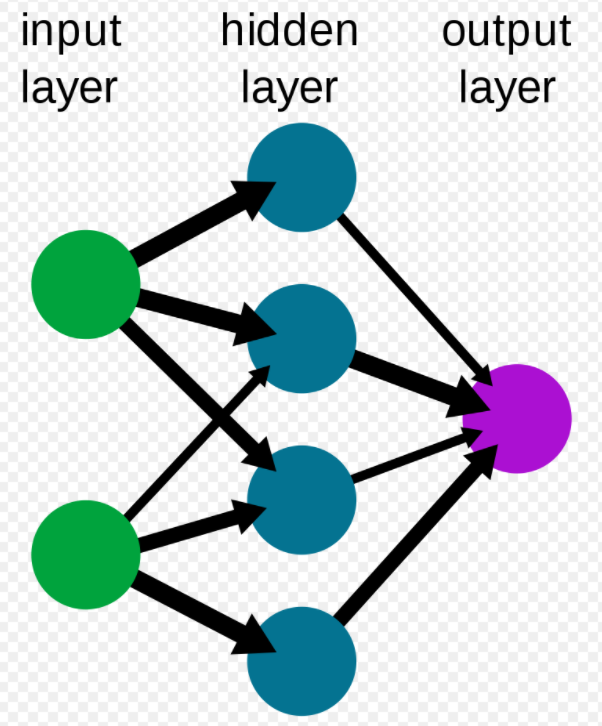
\includegraphics[width=6cm]{FFNN.png}\caption{Neural Network Architecture}\end{figure}

\newpage
\subsubsection{Neural Network - Function definitions}
\begin{itemize}
	\item Affine layer $y = Ax + b , x \in \mathbb{R}^n, b, y \in \mathbb{R}^m, A \in \mathbb{R}^{m \times n}$
	\item Activation point wise
	\begin{itemize}
		\item $\sigma_g(z) = \frac{1}{1+e^{-z}}$ - Sigmoid 
		\item $ReLU(z) = \max(0, z)$  - Rectified linear unit
	\end{itemize}	
\end{itemize}

\begin{figure}[H]\centering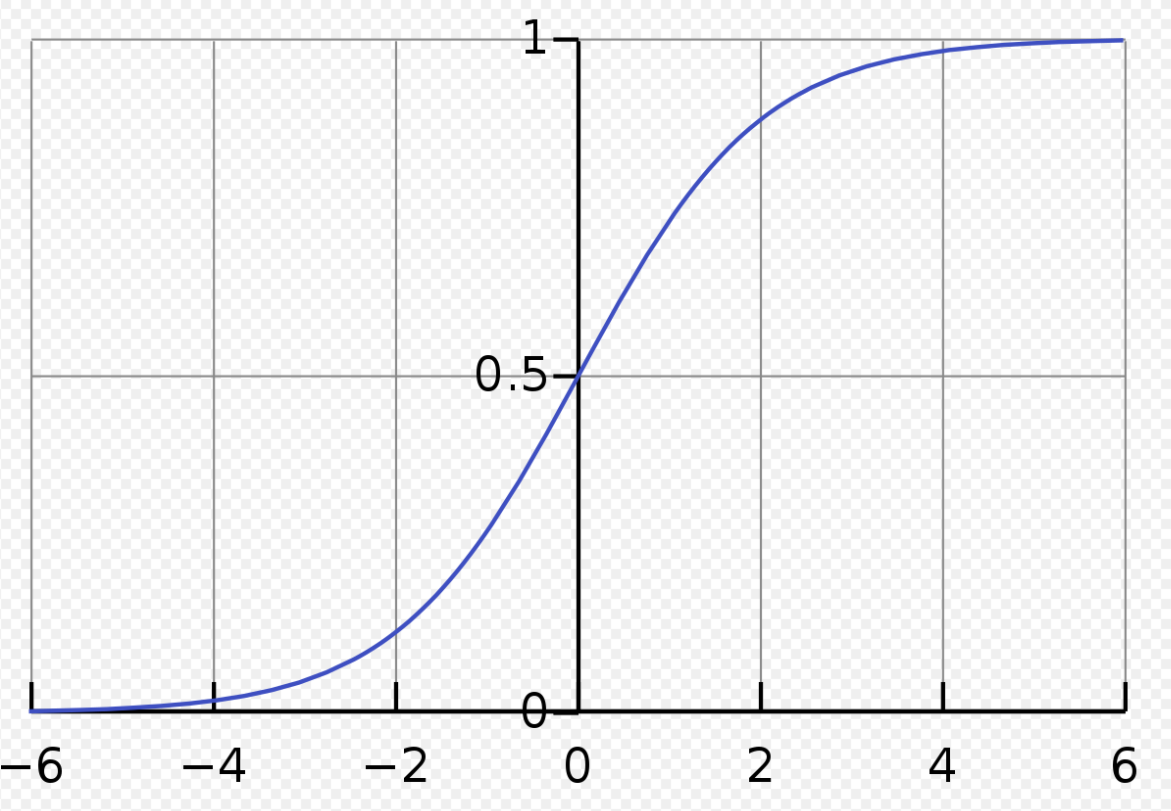
\includegraphics[width=6cm]{sigmoid.png}\caption{Sigmoid function}\end{figure}
\begin{figure}[H]\centering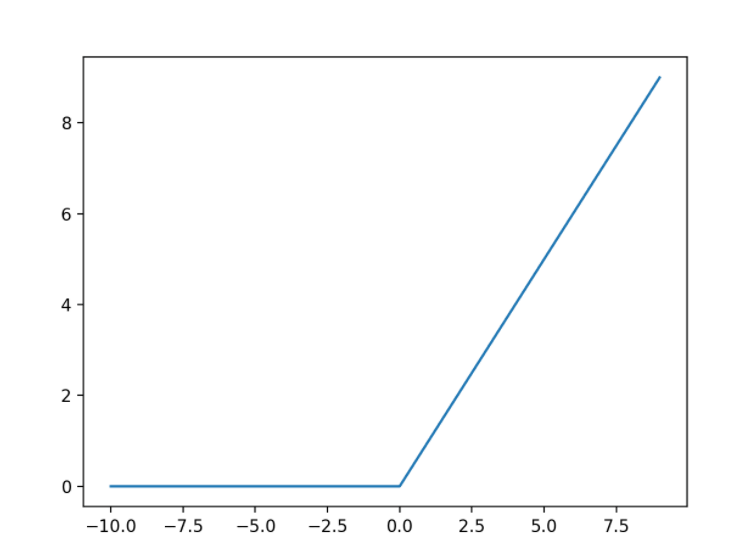
\includegraphics[width=6cm]{RELU.png}\caption{ReLU function}\end{figure}

\newpage
\subsubsection{Neural Network - Layering functions}

\begin{itemize}
	\item Dense: $y = \sigma(L), L = Ax+b$
	\item Expressiveness 
	\item Back propagation - $\frac{\partial y}{ \partial w} =  \frac{\partial y}{ \partial L} \cdot \frac{\partial L}{ \partial w}$
\end{itemize}


\subsubsection{Neural Network - Hyperbolic tangent  function}
$\sigma_h = \tanh(z) = \frac{e^z-e^{-z}}{e^z+e^{-z}}$
\begin{figure}[H]\centering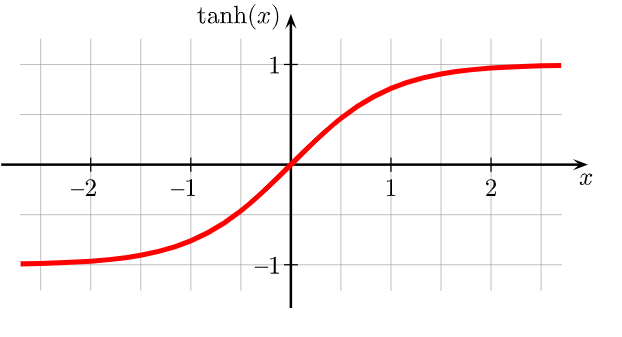
\includegraphics[width=6cm]{tanh.png}\caption{Hyperbolic tangent function}\end{figure}


\subsubsection{Neural Network - Problems}


\begin{itemize}
	\item Fixed size input
	\item No memory
\end{itemize}


\newpage
\subsection{RNN}

\subsubsection{RNN - Introduction}
\begin{itemize}
	\item Signals with timestamp (time series) - $\{x_t, y_t \}_{t=1}^k$
	\item Hidden state - $h_t = f_{W}(x_t, h_{t-1})$
	\item Same weights $W$ for each step
	\item Popular in Natural Language Processing (NLP)
\end{itemize}
\begin{figure}[H]\centering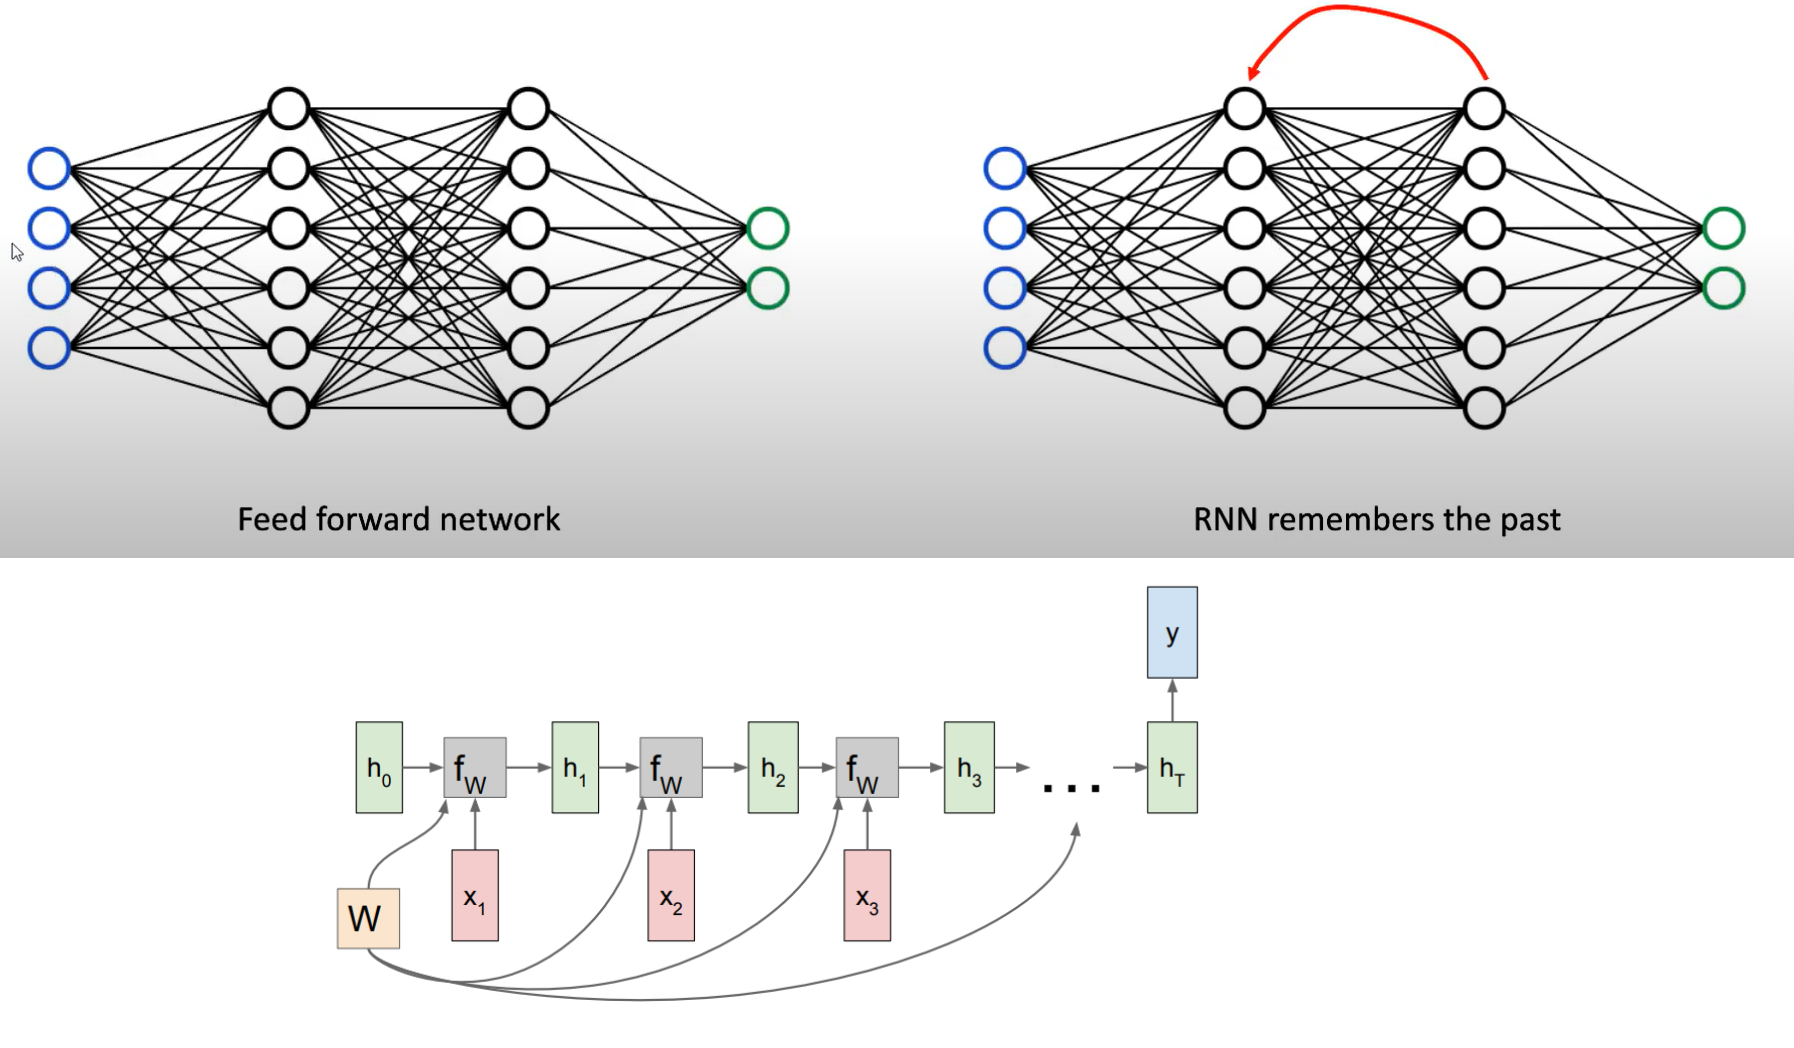
\includegraphics[width=10cm]{RNN.png}\caption{RNN}\end{figure}


\subsubsection{RNN - Simple example}

\begin{itemize}
	\item $h_t = \sigma_h \big(W_{hh} h_{t-1} +  W_{xh} x_{t} + b_h\big)$
	\item $y_t  = W_{hy} h_{t} +  b_y$
\end{itemize}

\subsubsection{RNN - Multi-Layer}
\begin{figure}[H]\centering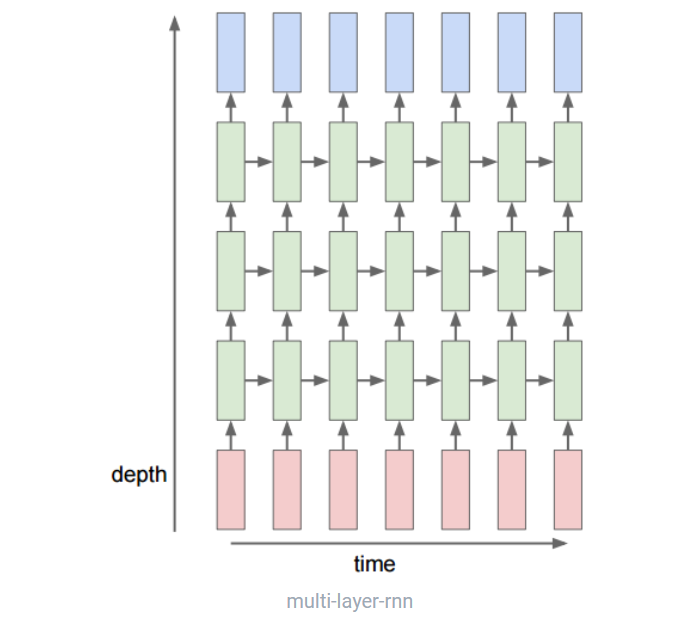
\includegraphics[width=10cm]{RNN_MULTI.png}\caption{RNN - MultiLayer}\end{figure}
\begin{align*}
	h_t^{layer} = \sigma_h \bigg(W^{layer} \begin{pmatrix}
		h_{t}^{layer-1} \\ h_{t-1}^{layer}
	\end{pmatrix} \bigg)
\end{align*}


\subsubsection{RNN - Training }
Back propagation through time:
\begin{figure}[H]\centering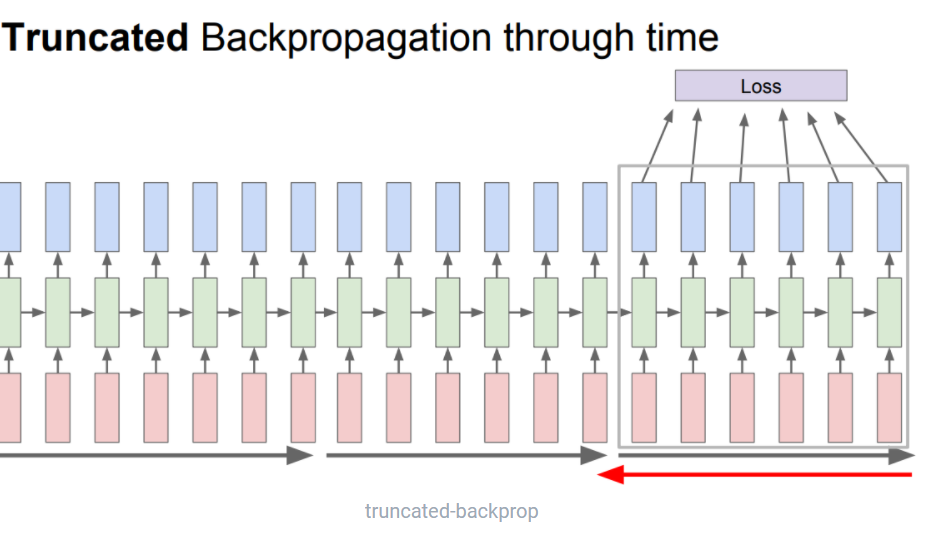
\includegraphics[width=10cm]{RNN_BACKPROP.png}\caption{RNN - back propagation}\end{figure}


\subsubsection{RNN - Problems}

Small example, scalars and no hidden states:
\begin{figure}[H]\centering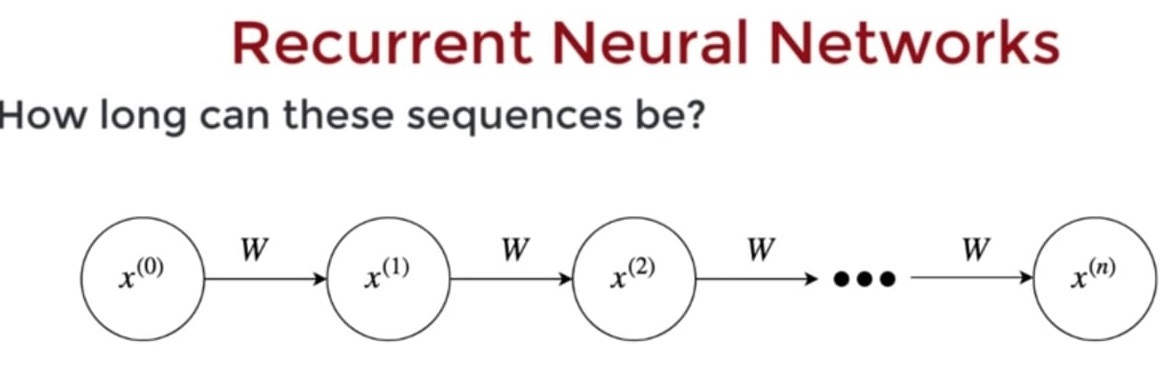
\includegraphics[width=10cm]{Explode.jpeg}\caption{RNN - Exploding vanishing gradients}\end{figure}

\begin{itemize}
	\item Exploding vanishing gradients
	\item $x^{(n)} = W^t x^{(0)}$
	\item 10 time steps.
\end{itemize}

\newpage
\subsection{LSTM}


\subsubsection{LSTM - Motivation}

LSTM (Long Short Term Memory) is a special kind of RNN,  designed to overcome the limitation of RNN
\begin{itemize}
	\item Gradient vanishing and exploding
	\item Complex training
	\item Difficulty to processes long sequences 
\end{itemize}

Remembering information for long periods of time is intrinsic to LSTM.

\subsubsection{LSTM - Principles}


\begin{figure}[H]\centering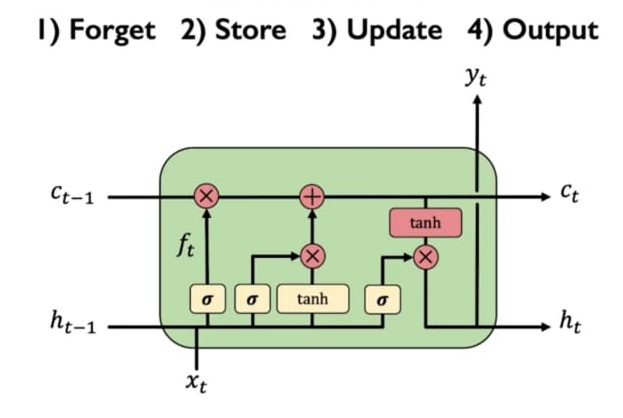
\includegraphics[width=7.5cm]{LSTM_MAIN.jpeg}\caption{LSTM - Scheme}\end{figure}

\begin{figure}[H]\centering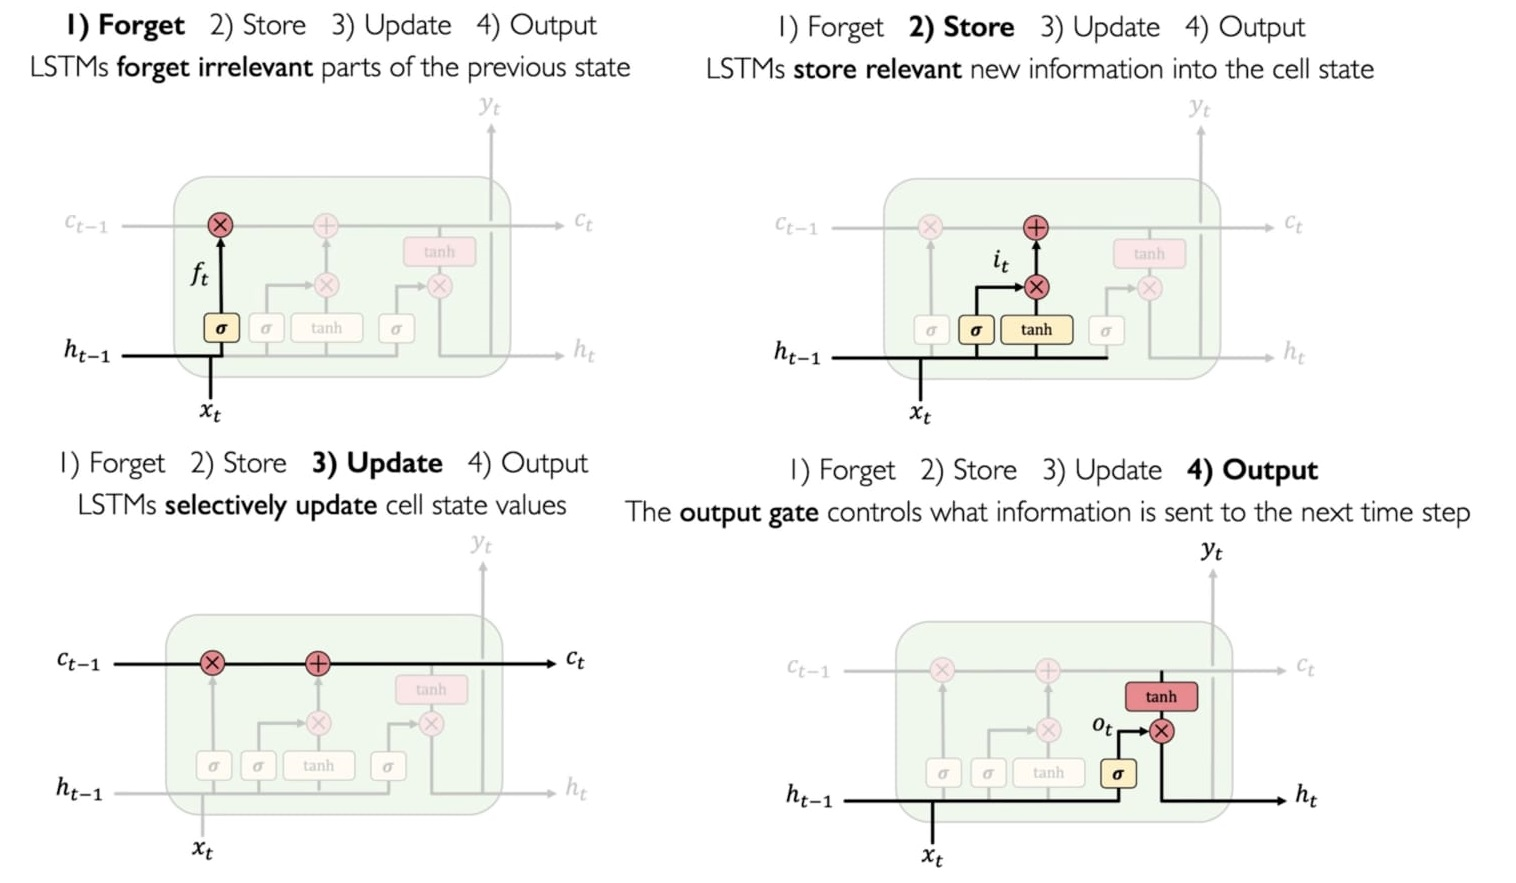
\includegraphics[width=14cm]{LSTM_SCHEME.jpeg}\caption{LSTM - Scheme}\end{figure}

\begin{itemize}
	\item Separate Cell state
	\item Gate to control flow of information:
	\begin{itemize}
		\item \textbf{Forget} - Gets rids of irrelevant information.
		\item \textbf{Store} - Relevant information from input
		\item \textbf{Update} - Selectively update cell state
		\item \textbf{Output}
	\end{itemize}
\end{itemize}


\begin{figure}[H]\centering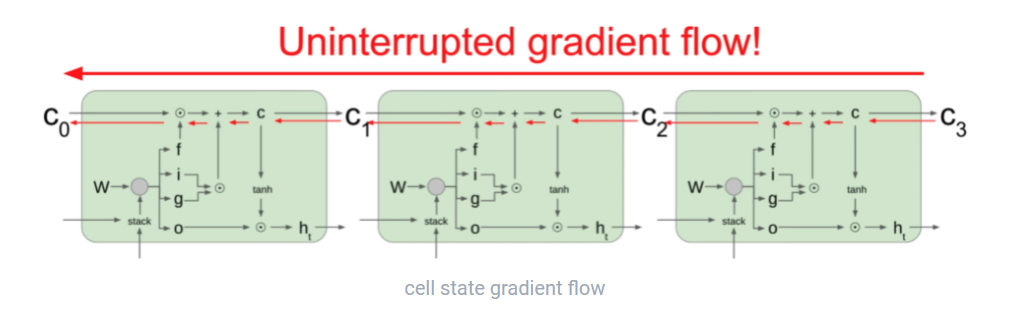
\includegraphics[width=10cm]{LSTM_GRADIENT_FLOW.png}\caption{LSTM - Gradient flow}\end{figure}


\subsubsection{LSTM- Formulation}
\begin{align*}
	f_t &= \sigma_g(W_{f} x_t + U_{f} h_{t-1} + b_f) \\
	i_t &= \sigma_g(W_{i} x_t + U_{i} h_{t-1} + b_i) \\
	o_t &= \sigma_g(W_{o} x_t + U_{o} h_{t-1} + b_o) \\
	\tilde{c}_t &= \sigma_c(W_{c} x_t + U_{c} h_{t-1} + b_c) \\
	c_t &= f_t \circ c_{t-1} + i_t \circ \tilde{c}_t \\
	h_t &= o_t \circ \sigma_h(c_t)
\end{align*}

where the initial values are $c_0 = 0$ and $h_0 = 0$ and the operator $\circ$ denotes the Hadamard product (element-wise product). 

\begin{itemize}
	\item $x_t \in \mathbb{R}^{d}$: input vector to the LSTM unit 
	\item $f_t \in \mathbb{R}^{h}$: forget gate's activation vector
	\item $i_t \in \mathbb{R}^{h}$: input/update gate's activation vector 
	\item $o_t \in \mathbb{R}^{h}$: output gate's activation vector
	\item $h_t \in \mathbb{R}^{h}$: hidden state vector also known as output vector of the LSTM unit 
	\item $\tilde{c}_t \in \mathbb{R}^{h}$: cell input activation vector
	\item $c_t \in \mathbb{R}^{h}$: cell state vector
	\item $W \in \mathbb{R}^{h \times d}, U \in \mathbb{R}^{h \times h} $ and $b \in \mathbb{R}^{h}$: weight matrices and bias vector parameters which need to be learned during training
\end{itemize}

where the superscripts $d$ and $h$ refer to the number of input features and number of hidden units, respectively.


\subsubsection{LSTM- Multi-cell}

\begin{figure}[H]\centering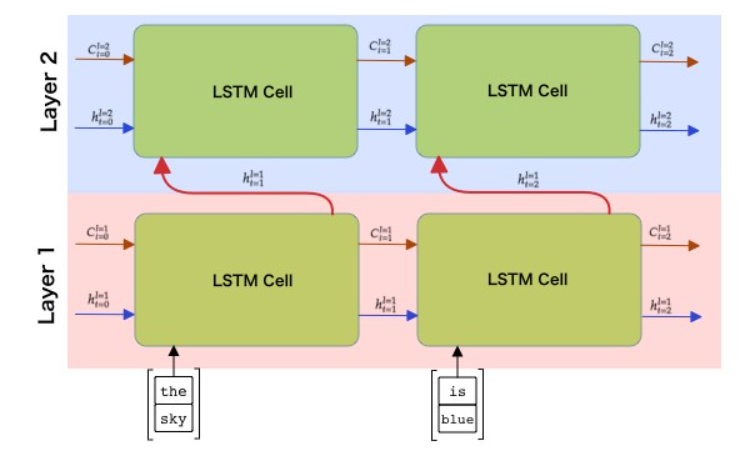
\includegraphics[width=10cm]{LSTM_MULTI.png}\caption{LSTM - Multi layer cells}\end{figure}
\subsubsection{LSTM - in context of rainfall}

\begin{itemize}
	\item 2018
	\begin{itemize}
		\item CAMELS - Data set
		\item 2-Layer LSTM -cells
		\item Input feature size $d=5$ - prcp(mm/day), srad(W/m2), tmax(C), tmin(C), vp(Pa). 
		\item Hidden state  size $h=20$
		\item Dropout rate = $10\%$
		\item Sequemce length - $365$ days. 
	\end{itemize} 
	\item 2019
	\begin{itemize}
		\item CAMELS - Data set
		\item 1-Layer LSTM 
		\item Input feature size $d=5$ ? 
		\item Hidden state  size $h=256$
		\item Dropout rate = $40\%$
		\item Sequence length - $270$ days. 
	\end{itemize} 	
\end{itemize}

\newpage






\chapter{Results} 
 
\section{Sanity Check}

\section{Dream synthetic model}

\section{CelebA data set}

\section{Caravan Data set}


\chapter{Discussions} 

\chapter{Conclusions} 

















\newpage


$S_{b_1} = \big\{X_i, Y_i\big\}_{i=1}^{i=n_1}\quad , X_i,Y_i \sim f(X,Y| b_1) $  \\ \\
$S_{b_2} = \big\{X_i, Y_i\big\}_{i=1}^{i=n_2}\quad , X_i,Y_i \sim f(X,Y| b_2) $ \\

$S_{b_1} \cup S_{b_2}$ \\

$X$ \\ $Y$ \\ $ \big\{b_1, b_2\big\}$ \\ \\ 

$\text{Trained Model} \mapsto \text{Interpetabilty attributes}$ \\
$attributes_{\{S_{b_1} \cup S_{b_2}\}}$

	
\newpage

\printbibliography



\end{document}
